\documentclass[12pt,letter]{article}
\usepackage{mathptmx} % added for time new roman font
\usepackage[left=1in,right=1in,top=1in,bottom=1in]{geometry}
\usepackage[latin1]{inputenc}
\usepackage{amsmath}

% defines all example enviorment
\usepackage[framemethod=tikz]{mdframed} % added for the box around examples
\newtheorem{ex}{Example}
\numberwithin{ex}{section} % allows for the use of example numbers that lign up with the section numbers
\newenvironment{example}{\begin{mdframed}[middlelinewidth=0.5mm]\begin{ex}\normalfont}{\end{ex}\end{mdframed}}

% defines all review enviorment
\usepackage[framemethod=tikz]{mdframed} % added for the box around examples
\newtheorem{re}{Review}
\numberwithin{re}{section} % allows for the use of example numbers that lign up with the section numbers
\newenvironment{review}{\begin{mdframed}[middlelinewidth=2mm,roundcorner=20pt]\begin{re}\normalfont}{\end{re}\end{mdframed}}

% defines the quotation enviorment 
\usepackage{xcolor}
\newcommand{\quotebox}[2]{\begin{center}\fcolorbox{white}{blue!15!gray!15}{\begin{minipage}{0.9\linewidth}\vspace{10pt}\center\begin{minipage}{0.8\linewidth}{\space\Huge``}{#1}{\Huge''}{\break\null\hfill} {\small #2}  \end{minipage}\medbreak\end{minipage}}\end{center}}

% defines the definition enviorment 
\newcommand{\definitionbox}[2]{\begin{center}\fcolorbox{white}{blue!15!gray!15}{\begin{minipage}{0.9\linewidth}\vspace{10pt}\center\begin{minipage}{0.8\linewidth} {{\textbf{Definition} - }{#1}: {#2}}\end{minipage}\medbreak\end{minipage}}\end{center}}

\usepackage{amsfonts}
\usepackage{amssymb}
\usepackage{graphicx}
\usepackage{float}
\usepackage{booktabs}
%\usepackage{parskip} % remove all the paragraph indents
\usepackage[textsize=tiny]{todonotes}


\usepackage{setspace}
\usepackage[colorlinks=true]{hyperref}
\usepackage{textcomp} 
\usepackage{multicol} 

% added for MATLAB code
\usepackage[framed]{matlab-prettifier}
\let\ph\mlplaceholder % shorter macro
\lstMakeShortInline"

\lstset{
  style              = Matlab-editor,
  basicstyle         = \mlttfamily,
  escapechar         = ",
  mlshowsectionrules = true,
}



\usepackage{color} % color added for editing
\newcommand{\bl}[1]{\textcolor[rgb]{0.00,0.00,1.00}{#1}}
\newcommand{\gr}[1]{\textcolor[rgb]{0.00,0.50,0.00}{#1}}
\newcommand{\rd}[1]{\textcolor[rgb]{0.75,0.00,0.00}{#1}}
\newcommand{\tl}[1]{\textcolor[rgb]{0,0.6,0.60}{#1}}



%%%%%%%		define the symbols for positive directions		%%%%%%
\makeatletter													%%	
																%%					
\newcommand*\curveplus{% positive counterclockwise				%%
  \mathbin{\rotatebox[origin=c]{90}{$\m@th\curvearrowleft$}+}}	%%
																%%
\newcommand*\rightplus{% positive right							%%
  \mathpalette\@rightplus\relax}								%%
\newcommand*\@rightplus[1]{%									%%
  \mathbin{\vcenter{\hbox{$\m@th\overset{#1+}{\to}$}}}}			%%
																%%	
\newcommand*\upplus{% positive up								%%
  \mathbin{+\mathord\uparrow}}									%%
																%%			
\newcommand*\downplus{% positive down							%%		
  \mathbin{+\mathord\downarrow}}								%%
  																%%		
\newcommand*\downrightplus{% positive down and right			%%	
  \mathbin{+ \rotatebox[origin=c]{-30}{$\m@th\rightarrow$}}}	%%
\makeatother 													%%	
%%%%%%%%%%%%%%%%%%%%%%%%%%%%%%%%%%%%%%%%%%%%%%%%%%%%%%%%%%%%%%%%%%


\usepackage{mathtools}          %loads amsmath as well added for the piece wise function
\DeclarePairedDelimiter\Floor\lfloor\rfloor
\DeclarePairedDelimiter\Ceil\lceil\rceil

 
\newcounter{NumberInTable}
\newcommand{\LTNUM}{\stepcounter{NumberInTable}{(\theNumberInTable)}}

\newcommand{\Laplace}[1]{\ensuremath{\mathcal{L}{\left[#1\right]}}}
\newcommand{\InvLap}[1]{\ensuremath{\mathcal{L}^{-1}{\left[#1\right]}}}
\renewcommand{\textuparrow}{$\uparrow$}


\begin{document}
	
	% set the section number, along with figure and equation numbers
	\setcounter{section}{2}	
	\setcounter{figure}{0}   
	\renewcommand\thefigure{\thesection.\arabic{figure}}
	\setcounter{equation}{0}   
	\renewcommand\theequation{\thesection.\arabic{equation}}

	\section{Forced Vibrations}


		

			Mechanical systems are ofter subjected to an external loading. For example, a piston in a engine if forced up and down my a crankshaft or a seat in an airplane my vibrate due to movement of the jet engines transmitted through the aircraft structure. 
			
		\subsection{Harmonic Excitations of Undamped Systems}
		
			\todo{I may have an issue where the radicand of the damped natural frequency is 1-2$\zeta^2$.}

			
			Investigating a single-degree of freedom system for a harmonic input is a useful as it can be solved mathematically with straightforward techniques. Consider the system:
			\begin{figure}[H]
				\centering
				\includegraphics[]{../figures/1-DOF-spring_mass_horizontal_forced_FBD.png}
				\caption{1-DOF system with an external force ($F(t)$) applied, showing: (a) the system configuration; and (b) the free body diagram}
				\label{fig:1-DOF-spring_mass_horizontal_forced_FBD}
			\end{figure}	
			\noindent where $F(t)$ is the external force applied to the mass. For simplicity, let us consider a harmonic excitation for $F(t)$ such that:
			\begin{equation}
				F(t) = F_0\text{cos}(\omega t)
			\end{equation}							
			note that here, $\omega$ has no subscript and is the frequency in rad/sec of the driving force. $F_0$ represents the magnitude of the applied force. This is often called the input frequency, driving frequency, or forcing frequency. Building the EOM for system in figure \ref{fig:1-DOF-spring_mass_horizontal_forced_FBD} yields:
			\begin{equation}
				m \ddot{x}(t)+kx(t) = F_0\text{cos}(\omega t)
			\end{equation}			
			For convenience we drop the ``$(t)$'' to make the writing easier. Then, we convert the EOM to the standard form by dividing the equation through by $m$:					
			\begin{equation}
				\ddot{x}+\omega_n^2x = f_0\text{cos}(\omega t)
			\end{equation}					
			where:
			\begin{equation}
				f_0 = \frac{F_0}{m}
			\end{equation}	
			The EOM in this form is a second order, linear nonhomogeneous differential equation. It is nonhomogeneous because there are no terms related to $x$ on the right-hand side of the equation. One way to solve such such an ODE is to recall that the solution for a nonhomogeneous equation is the sum of the homogeneous and particular solutions. 
			\begin{equation}
				x = x_h + x_p
			\end{equation}	
			again, noting that this is a temporal solution where ``$(t)$'' is implied. First, knowing that the solution is the sum of two parts: 1) oscillations caused by the spring/mass system; and 2) vibrations caused by the forcing function. The oscillations caused by the spring/mass system will form the homogeneous while the vibrations caused by the forcing function will form the particular solution. As we know the solution for oscillations caused by the spring/mass system form our prior investigation of unforced system we set the equation for the homogeneous solution to be:
			\begin{equation}
				x_h = A\text{sin}(\omega_n t + \phi)
			\end{equation}			
			Next, we will denote the particular solution as $x_p$. $x_p$ can be determined by assuming that it is in form of the forcing function, therefore:
			\begin{equation}
				f_0\text{cos}(\omega t)
			\end{equation}	
			becomes:
			\begin{equation}
				x_p  =X\text{cos}(\omega t)
			\end{equation}						
			where, $x_p$ is the particular solution and $X$ is the amplitude of the forced response. Our total solution for the harmonic excitations of undamped systems now becomes:
			\begin{equation}
				x(t) = A\text{sin}(\omega_n t + \phi) + X\text{cos}(\omega t) 
			\end{equation}				
			This approach, of assuming that $x_p=X\text{cos}(\omega t)$, in order to determine the particular solution is called the \textbf{method of undetermined coefficients}. To calculate $X$, first we take the equations for $x_p$ and $\ddot{x}_p $:
			\begin{equation}
				x_p = X\text{cos}(\omega t)
			\end{equation}	
			\begin{equation}
				\ddot{x}_p = -\omega^2X\text{cos}(\omega t)
			\end{equation}				
			and substituting these into the equation of motion in standard from yields:
			\begin{equation}
				-\omega^2X\text{cos}(\omega t)+\omega_n^2X\text{cos}(\omega t) = f_0\text{cos}(\omega t)
			\end{equation}		
			As long as 	$\text{cos}(\omega t) \neq  0$, solving for X yields:
			\begin{equation}
				X = \frac{f_0}{\omega_n^2-\omega^2}
				\label{eq:X}
			\end{equation}		
			Therefore, as long as $\omega_n \neq \omega$, the particular solution can take the form:
			\begin{equation}
				x_p = \frac{f_0}{\omega_n^2-\omega^2}\text{cos}(\omega t)
			\end{equation}						
			This then expands to the total form:
			\begin{equation}
				x(t) = A\text{sin}(\omega_n t + \phi) + \frac{f_0}{\omega_n^2-\omega^2}\text{cos}(\omega t)
			\end{equation}				
			Expanding this to the general form for the homogeneous solution obtains the equation:
			\begin{equation}
				x(t) = A_1\text{sin}(\omega_n t) + A_2\text{cos}(\omega_n t) + \frac{f_0}{\omega_n^2-\omega^2}\text{cos}(\omega t)
			\end{equation}				
			As before, we need to determine the values for the coefficients $A_1$ and $A_2$ by enforcing the initial conditions $x_0$ and $v_0$. Setting the time to zero ($t=0$) and solving the initial displacement leads to:
			\begin{equation}
				x(0) = x_0 = A_2 + \frac{f_0}{\omega_n^2-\omega^2}
			\end{equation}				
			or:
			\begin{equation}
				A_2 = x_0-\frac{f_0}{\omega_n^2-\omega^2}
			\end{equation}	
			again, solving the equation in terms of velocity:
			\begin{equation}
				\dot{x}(t) = A_1\omega_n\text{cos}(\omega_n t) - A_2 \omega_n \text{sin}(\omega_n t) - \omega \frac{f_0}{\omega_n^2-\omega^2}\text{sin}(\omega t)
			\end{equation}	
			and solving for the initial velocity at $t=0$:
			\begin{equation}
				\dot{x}(0) = v_0 =  A_1 \omega_n
			\end{equation}				
			or:
			\begin{equation}
				A_1 = \frac{v_0}{\omega_n}
			\end{equation}				
			Therefore, combining the equations we get:
			\begin{equation}
				x(t) = \Big(\frac{v_0}{\omega_n}\Big)\text{sin}(\omega_n t) + \Big(x_0-\frac{f_0}{\omega_n^2-\omega^2}\Big)\text{cos}(\omega_n t) + \frac{f_0}{\omega_n^2-\omega^2}\text{cos}(\omega t)
			\end{equation}	
			As before, we can relate $A_1$ and $A_2$ to each other through the basic trigonometric identities. This yields, 
			\begin{equation}
				x(t) = A\text{sin}(\omega_n t + \phi) + X\text{cos}(\omega t) 
			\end{equation}				
			\begin{equation}
				A = \sqrt{\bigg(\frac{v_0}{\omega_n}\bigg)^2+(x_0-X)^2}
			\end{equation}				
			\begin{equation}
				\phi = \text{tan}^{-1}\bigg(\frac{\omega_n(x_0-X)}{v_0}\bigg)
			\end{equation}				
			\begin{equation}
				X = \frac{f_0}{\omega_n^2-\omega^2}
			\end{equation}				
			
			\begin{example}
				For a the 1-DOF system:
				\begin{figure}[H]
					\centering
					\includegraphics[width=0.5\textwidth]{../figures/1-DOF-spring_mass_horizontal_forced.png}
					\caption{1-DOF spring-mass system subjected to an external force $F(t)$.}
				\end{figure}
				with with $k$ = 10 N/m, $m$ = 2.5 kg, $\omega$ = 4 rad/sec, $F_0$ = 0.1 kN, $x_0$ = 1 mm, and $v_0$ = 0 mm plot the temporal responses of system considering the free-vibration case and the excited case. Plot these on a single plot to compare the responses. 
							
				\noindent\textbf{Solution:} The free-vibration response can be plotted using the expression:
				\begin{equation}
					x(t) = x_0\text{cos}(\omega_n t) + \frac{v_0}{\omega_n}\text{sin}(\omega_n t)
				\end{equation}				
				while the force vibration is expressed using:
				\begin{equation}
					x(t) = \Big(\frac{v_0}{\omega_n}\Big)\text{sin}(\omega_n t) + \Big(x_0-\frac{f_0}{\omega_n^2-\omega^2}\Big)\text{cos}(\omega_n t) + \frac{f_0}{\omega_n^2-\omega^2}\text{cos}(\omega t)
				\end{equation}	
				These temporal responses are plotted as (Note that the forcing function uses the axis on the right):
				\begin{figure}[H]
					\centering
					\includegraphics[width=0.9\textwidth]{../figures/free_and_forced_temporal_response.png}
					\caption{Comparison of the temporal response for a 1-DOF system; expressing how the forcing function changes the vibrational  temporal response of the system.}
				\end{figure}	
			\end{example}
			
			
		\subsection{Harmonic Resonance}			
			
			Recall that our solution from before assumed that $\omega_n \neq \omega$, however, if $\omega_n = \omega$ then the system will develop the phenomenon of resonance. Mathematically, this means the amplitude of the vibrations becomes unbounded. The prior choice of $X\text{cos}(\omega t)$ for the particular solution fails as it is also a solution for a homogeneous equation. Therefore, a new particular solution is needed for the case where $\omega_n = \omega$. This new particular solution can be written as:
			\begin{equation}
				x_p(t) = t X\text{sin}(\omega t)
			\end{equation}				
			Substituting this into the EOM of the system in standard form equation (from Boyce and DiPrima (1997)) and solving for X yields:
			\begin{equation}
				x_p(t) = \frac{f_0}{2 \omega} t \text{sin}(\omega t)
			\end{equation}	
			thus, the total solution can now be written as:
			\begin{equation}
				x(t) = A_1\text{sin}(\omega t) + A_2\text{cos}(\omega t) + \frac{f_0}{2 \omega} t \text{sin}(\omega t)
			\end{equation}			
			Note that $\omega_n=\omega$, therefore, the frequencies are all in terms of the driving frequency $\omega$. Again, evaluating the solution at $t=0$ for the initial conditions $x_0$ and $v_0$ yields:
			\begin{equation}
				x(t) = \Big(\frac{v_0}{\omega}\Big)\text{sin}(\omega t) + x_0\text{cos}(\omega t) + \frac{f_0}{2 \omega} t \text{sin}(\omega t)
			\end{equation}			
			Where the first two terms account for the oscillations while the third terms accounts for the continued increase of the maximum amplitude. The following plot shows the forced response of a spring-mass system driven harmonically at its natural frequency.
			\begin{figure}[H]
				\centering
				\includegraphics[]{../figures/resonance.png}
			\end{figure}				

\begin{example}

			Compute solutions for the homogeneous and particular solution separately, than compute the total response of a spring-mass system with the following values: $k$ = 1000 N/m, $m$ = 10 kg, subject to a harmonic force of magnitude $F_0$ = 100 N and frequency of 8.162 rad/s, and initial conditions given by $x_0$ = 0 m and $v_0$ = 0 m/s. Plot the response.
			
			\begin{figure}[H]
				\centering
				\includegraphics[width=0.5\textwidth]{../figures/1-DOF-spring_mass_horizontal_forced.png}
				\caption{1-DOF spring-mass system subjected to an external force $F(t)$.}
			\end{figure}
			
			\noindent\textbf{Solution:} First, make sure that the system is not in resonance. Calculating that $\omega_n = \sqrt{1000/10} = 10$ shows us that $\omega_n \neq \omega$. Next knowing that $f_0 = F_o/m = 10$ we can find the homogeneous and particular solutions as:
			\begin{equation}
				x_h(t) = A\text{sin}(\omega_n t + \phi)
			\end{equation}				
			\begin{equation}
				x_p(t) = X\text{cos}(\omega t) 
			\end{equation}	
			also:			
			\begin{equation}
				x(t) = x_h(t) + x_p(t)
			\end{equation}	
			where:			
			\begin{equation}
				A = \sqrt{\bigg(\frac{v_0}{\omega_n}\bigg)^2+(x_0-X)^2} = 
			\end{equation}				
			\begin{equation}
				\phi = \text{tan}^{-1}\bigg(\frac{\omega_n(x_0-X)}{v_0}\bigg)
			\end{equation}				
			\begin{equation}
				X = \frac{f_0}{\omega_n^2-\omega^2}
			\end{equation}			
			This leads to the following results. 
			\begin{figure}[H]
				\centering
				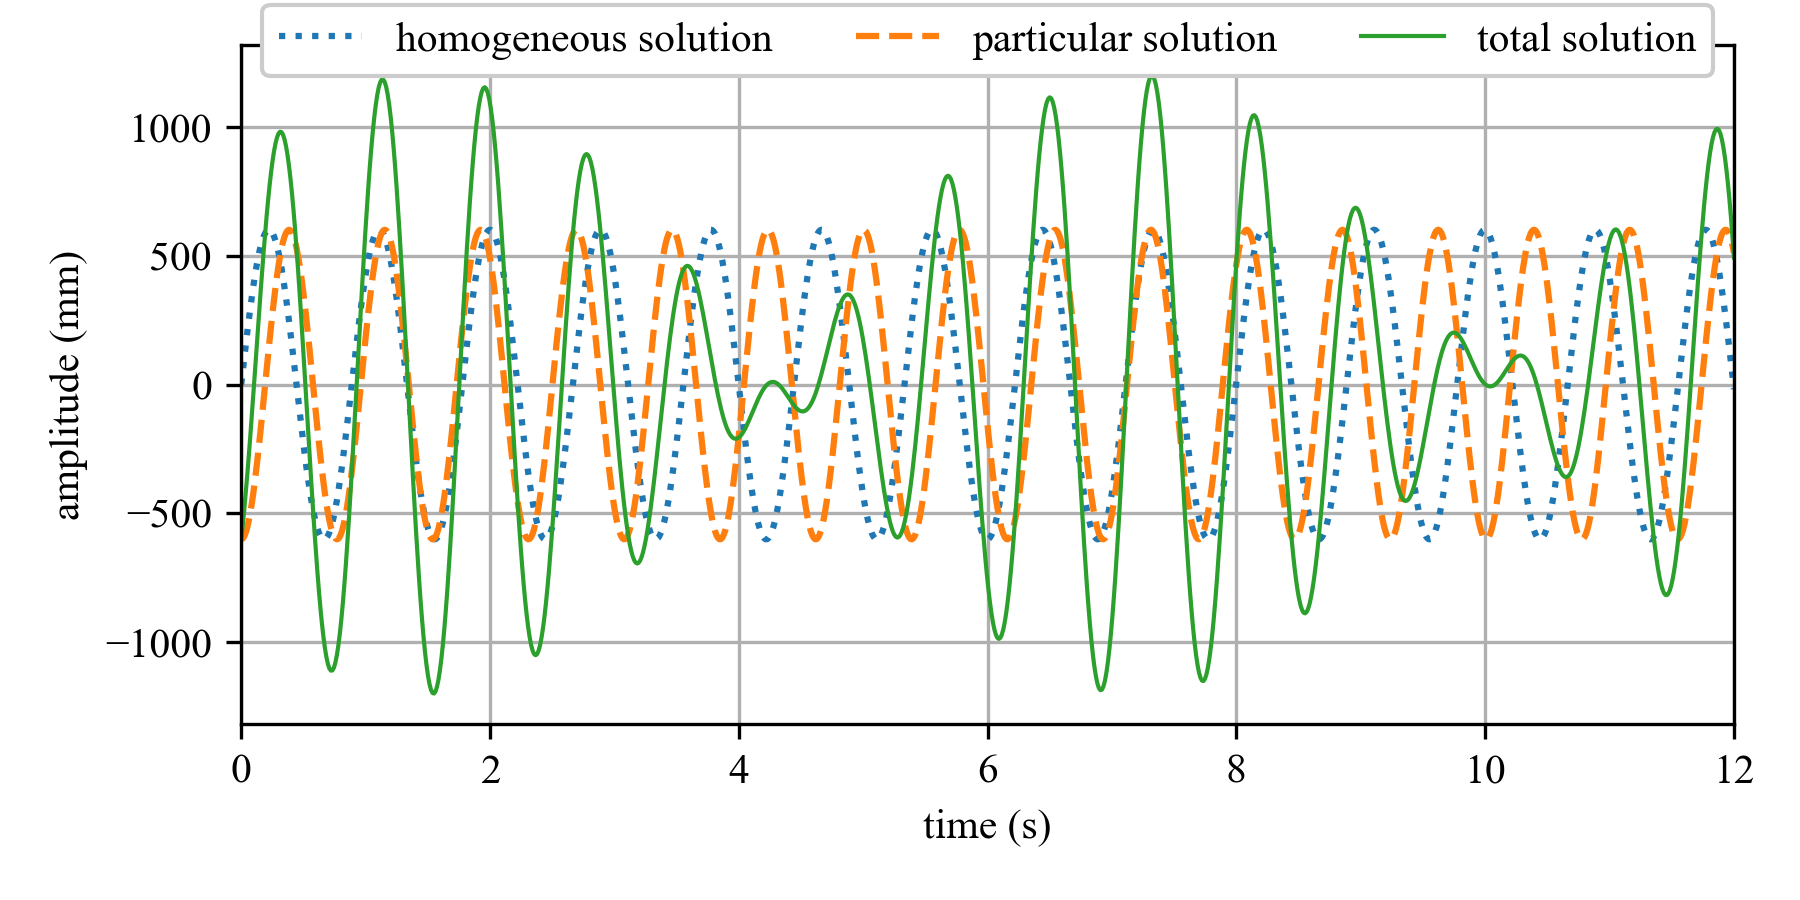
\includegraphics[]{../figures/homogeneous_and_particular_solutions.png}
			\end{figure}			

\end{example}

\begin{example}
			Considering the following system, write the equation of motion and calculate the response assuming a) that the system is initially at rest, and b) that the system has an initial displacement of 0.005 m. Use $k$ = 2000 N/m, $m$ = 100 kg, $F(t)$ = 10sin(10t) N.
			\begin{figure}[H]
				\centering
				\includegraphics[width=0.5\textwidth]{../figures/1-DOF-spring_mass_horizontal_forced.png}
				\caption{1-DOF spring-mass system subjected to an external force $F(t)$.}
			\end{figure}
			\noindent\textbf{Solution:} The equation of motion is
			\begin{equation}
				m\ddot{x}+kx=10\text{sin}(10t)
			\end{equation}
			or in standard form:
			\begin{equation}
				\ddot{x}+\omega_n^2x=f_0\text{sin}(\omega t)
			\end{equation}							
			Note that the forcing function is in terms of sin, not cos as before, so we will have to resolve for the constants $A_1$ and $A_2$. Again, setting the particular solution to $x_p=X\text{sin}(\omega t)$ and solving for $X$ as before yields:
			\begin{equation}
				x(t) = A_1\text{sin}(\omega_n t) + A_2\text{cos}(\omega_n t) + \frac{f_0}{\omega_n^2-\omega^2}\text{sin}(\omega t)
			\end{equation}	
			Now we can solve for $A_1$ and $A_2$ by setting the initial conditions $x_0$ and $v_0$ to $t=0$. First, setting $t=0$ in the equation for $x(t)$ yields:
			\begin{equation}
				A_2 = x_0
			\end{equation}	
			Then, a function for the velocity of the system is obtained: 
			\begin{equation}
				\dot{x}(t) = v_0 = A_1\omega_n\text{cos}(\omega_n t) - A_2\omega_n\text{sin}(\omega_n t) + \omega\frac{f_0}{\omega_n^2-\omega^2}\text{cos}(\omega t)
			\end{equation}				
			This allows us to obtains:
			\begin{equation}
				A_1 = \frac{v_0}{\omega_n}-\frac{\omega}{\omega_n}\cdot \frac{f_0}{\omega_n^2-\omega^2}
			\end{equation}	
			at $t=0$. These lead to the full equation for the general solution:
			\begin{equation}
				x(t) = \Big(\frac{v_0}{\omega_n}-\frac{\omega}{\omega_n}\cdot \frac{f_0}{\omega_n^2-\omega^2}\Big)\text{sin}(\omega_n t) + x_0\text{cos}(\omega_n t) + \frac{f_0}{\omega_n^2-\omega^2}\text{sin}(\omega t)
			\end{equation}								
			Also, knowing:
			\begin{equation}
				\omega_n = \sqrt{\frac{k}{m}} = \sqrt{20} \text{ rad/sec} =  4.472 \text{ rad/sec}
			\end{equation}				
			and
			\begin{equation}
				f_o = \frac{F_0}{m} = \frac{F_0}{m} = 0.1 \text{ N/kg}
			\end{equation}	
			a) using the initial conditions $x_0$ = 0 m and $v_0$ = 0 m/s and the general expression obtained above:
			\begin{equation}
				x(t) = \Big(0-\frac{10}{\sqrt{20}}\cdot \frac{0.1}{20-10^2}\Big)\text{sin}(\sqrt{20} t) + 0 + \frac{0.1}{20-10^2}\text{sin}(10 t)
			\end{equation}			
			b) using the initial conditions $x_0$ = 0.005 m and $v_0$ = 0 m/s and the general expression obtained above:
			\begin{equation}
				x(t) = \Big(0-\frac{10}{\sqrt{20}}\cdot \frac{0.1}{20-10^2}\Big)\text{sin}(\sqrt{20} t) + 0.05\text{cos}(\sqrt{20} t) + \frac{0.1}{20-10^2}\text{sin}(10 t)
			\end{equation}			
			\begin{figure}[H]
				\centering
				\includegraphics[width=1.0\textwidth]{../figures/response_1-DOF-spring_mass_forced.png}
			\end{figure}
\end{example}


	
		\subsection{Harmonic Excitations of Underdamped Systems}

			Consider the system:
			\begin{figure}[H]
				\centering
				\includegraphics[]{../figures/1-DOF-spring_dashpot_mass_horizontal_forced_FBD.png}
				\caption{Damped 1-DOF system with an external force ($F(t)$) applied, showing: (a) the system configuration; and (b) the free body diagram}
			\end{figure}	
			\noindent Again, for simplicity let us consider a harmonic excitation for $F(t)$ such that:
			\begin{equation}
				F(t) = F_0\text{cos}(\omega t)
			\end{equation}							
			Building the EOM for the above system results in:
			\begin{equation}
				m \ddot{x}(t)+c\dot{x}(t)+kx(t) = F_0\text{cos}(\omega t)
			\end{equation}			
			For convinces we can convert this to the standard form:					
			\begin{equation}
				\ddot{x}(t)+2 \zeta \omega_n \dot{x}(t) +\omega_n^2x(t) = f_0\text{cos}(\omega t)
			\end{equation}					
			again, where:
			\begin{equation}
				f_0 = \frac{F_0}{m}
			\end{equation}	
			Recall that one way to solve such an equation is to obtain the sum of the homogeneous and particular solutions. 
			\begin{equation}
				x(t) = x_h(t) + x_p(t)
			\end{equation}	
			However, now that we have damping force to consider, our particular solution will have to consider this damping. Therefore:
			\begin{equation}
				\label{eq:x_p(t)}
				x_p(t) = X \text{cos}(\omega t - \phi_p)
			\end{equation}
			where $\phi_p$ represents the phase shift. Note: $\phi_p$ is represented in other texts as $\theta$, $\theta_p$, or even just $\phi$ but we will use $\phi_p$ throughout the remainder of this text. Again, the phase shift is expected because of the effect of the damping force. Now, our total equation is:
			\begin{equation}
				x(t) = Ae^{-\zeta \omega_n t}\text{sin}(\omega_d t + \phi) +  X \text{cos}(\omega t - \phi_p)
			\end{equation}			
			We can use the method of undetermined coefficients to obtain $X$ and $\phi_p$ for the particular solution. First, considering that we write the particular solution in equivalent form:
			\begin{equation}
				x_p(t) = X \text{cos}(\omega t - \phi_p) = A_s \text{cos}(\omega t) + B_s  \text{sin}(\omega t)
			\end{equation}			 
			Taking the derivative of the assumed forms of the particular solution yields:
			\begin{equation}
				x_p(t) = A_s \text{cos}(\omega t) + B_s  \text{sin}(\omega t)
			\end{equation}	
			\begin{equation}
				\dot{x}_p(t) = -\omega A_s \text{sin}(\omega t) + \omega B_s  \text{cos}(\omega t)
			\end{equation}				 
			\begin{equation}
				\ddot{x}_p(t) = -\omega^2 A_s \text{cos}(\omega t) - \omega^2 B_s  \text{sin}(\omega t)
			\end{equation}				
			Recall that the homogeneous and particular solutions are each solutions on their own, therefor, the EOM can be used to describe just the particular solution. Substituting $x_p$. $\dot{x}_p$, and $\ddot{x}_p$ for $x$. $\dot{x}$, and $\ddot{x}$ in the EOM in standard form:
			\begin{equation}
			 	\ddot{x}+2 \zeta \omega_n \dot{x} +\omega_n^2x = f_0\text{cos}(\omega t)
			\end{equation}
			yields:
			\begin{equation}
			 	\big(	-\omega^2 A_s \text{cos}(\omega t) - \omega^2 B_s  \text{sin}(\omega t) \big)+2 \zeta \omega_n  \big( -\omega A_s \text{sin}(\omega t) + \omega B_s  \text{cos}(\omega t)  \big) +
			\end{equation}
			\begin{equation*}
				\omega_n^2 \big( A_s \text{cos}(\omega t) + B_s  \text{sin}(\omega t) \big) = f_0\text{cos}(\omega t)
			\end{equation*}				
			and rearranging in terms of sin($\omega t$) and cos($\omega t$) yields: 
			\begin{equation}
				(-\omega^2 A_s + 2 \zeta \omega_n \omega B_s + \omega_n^2 A_s -f_0) \text{cos}(\omega t) + 
			\end{equation}
			\begin{equation*}
				(-\omega^2 B_s - 2 \zeta \omega_n \omega A_s + \omega_n^2 B_s)\text{sin}(\omega t) =0
			\end{equation*}	
			From this expression it is clear that there are two special moments in time where cos($\omega t$) and sin($\omega t$) equal zero. First, considering that $t=\pi/(2\omega)$ results in cos($\omega t$)=0, sin($\omega t$)=1 and the equation simplifies to:
			\begin{equation}
				(-2\zeta \omega_n \omega)A_s + (\omega_n^2 - \omega^2)B_s = 0
			\end{equation}	
			Additionally, at $t=0$, sin($\omega t$)=0 and cos($\omega t$)=1. Therefore, the equation yields		
			\begin{equation}
				(\omega_n^2 - \omega^2)A_s + (2\zeta \omega_n \omega)B_s = f_0
			\end{equation}				
			We can solve two equations for two unknowns. Writing the two linear equations as the singular matrix equation yields:
			\begin{gather}
			   \begin{bmatrix}
			   \omega_n^2 - \omega^2 & 2\zeta \omega_n \omega \\
			   - 2\zeta \omega_n \omega &  \omega_n^2 - \omega^2
			   \end{bmatrix}
  			   \begin{bmatrix}
  			   A_s \\
  			   B_s
  			   \end{bmatrix}
			 = \begin{bmatrix} f_0 \\ 0
			 \end{bmatrix}
			\end{gather}
			This can be solved by computeing the complex inversing, to give us:
			\begin{equation}
				A_s = \frac{(\omega_n^2 - \omega^2)f_0}{(\omega_n^2 - \omega^2)^2 +  (2\zeta \omega_n \omega)^2}
			\end{equation}	
			\begin{equation}
				B_s = \frac{2\zeta \omega_n \omega f_0}{(\omega_n^2 - \omega^2)^2 +  (2\zeta \omega_n \omega)^2}
			\end{equation}	
			From trigonometric relationships we can see that, 
			\begin{equation}
				X = \sqrt{A_s^2 + B_s^2}
			\end{equation}	
			\begin{equation}
				\phi_p = \tan^{-1}\bigg(\frac{B_s}{A_s}\bigg)
			\end{equation}	
			We can now derive values for our particular solution $x_p$:
			\begin{equation}
				X = \frac{f_0}{\sqrt{(\omega_n^2 - \omega^2)^2 +  (2\zeta \omega_n \omega)^2}} 
				\label{eq:X_damped}
			\end{equation}	
			\begin{equation}
				\phi_p = \tan^{-1} \bigg(\frac{2\zeta \omega_n \omega}{\omega_n^2 - \omega^2}\bigg)
			\end{equation}				
			Now we can build a solution for the particular equation ($x_p$), therefore, the total solution becomes:
			\begin{equation}
				x(t) = x_h(t) + x_p(t)
			\end{equation}
			\begin{equation}
				x(t) = Ae^{-\zeta \omega_n t}\text{sin}(\omega_d t + \phi) +  X \text{cos}(\omega t - \phi_p)
			\end{equation}				
			Note for larger values of $t$, the homogeneous solution approaches zero resulting in the particular solution becoming the total solution. Therefore, the particular solution is sometimes called the steady state response and the homogeneous solution is called the transient response. Solving for the constants $A$ and $\phi$ using boundary conditions ($x_0=0$ and $v_0=0$) results a total solution expressed as:
			\begin{equation}
				A = \frac{x_0 -X \text{cos}(\phi_p)}{\text{sin}(\phi)}
			\end{equation}			 
			\begin{equation}
				\phi =  \tan^{-1} \bigg(\frac{\omega_d \big( x_0 -X \text{cos}(\phi_p)\big)}{v_0 + \big(x_0 - X \text{cos}(\phi_p)\big) \zeta \omega_n - \omega X \text{sin}(\phi_p) }\bigg)
			\end{equation}			
			Finally, assembling all the terms:
			\begin{equation}
				x(t) = Ae^{-\zeta \omega_n t}\text{sin}(\omega_d t + \phi) +  X \text{cos}(\omega t - \phi_p)
				\label{eq:damped_forced_x}
			\end{equation}
			\begin{equation}
				A = \frac{x_0 -X \text{cos}(\phi_p)}{\text{sin}(\phi)}
			\end{equation}			 
			\begin{equation}
				\phi =  \text{tan}^{-1}\bigg(\frac{\omega_d ( x_0 -X \text{cos}(\phi_p))}{v_0 + (x_0 - X \text{cos}(\phi_p)) \zeta \omega_n - \omega X \text{sin}(\phi_p) }\bigg)
			\end{equation}	
			\begin{equation}
				X = \frac{f_0}{\sqrt{(\omega_n^2 - \omega^2)^2 +  (2\zeta \omega_n \omega)^2}} 
			\end{equation}	
			\begin{equation}
				\phi_p = \tan^{-1} \bigg(\frac{2\zeta \omega_n \omega}{\omega_n^2 - \omega^2}\bigg)
				\label{eq:damped_forced_theta_p}
			\end{equation}		
			\begin{example}
			\label{ex:homogeneous_and_particular_solutions_in_resonance}		
				Consider the damped 1-DOF system below, plot the total, steady state, and transient responses for the following system configurations with no initial conditions. For each configuration, comment on the temporal response and how it differs from the response of the previous configuration.    
				
				\begin{itemize}
				\item[a)] $k=100$ N/m, $m=10$ kg,  $c=10$ kg/s, $F_0=1$ N, and $\omega = 8.162$.
				\item[b)] $k=100$ N/m, $m=10$ kg,  $c=10$ kg/s, $F_0=3$ N, and $\omega = 8.162$.
				\item[c)] $k=100$ N/m, $m=10$ kg,  $c=10$ kg/s, $F_0=3$ N, and $\omega = 3.162$.
				\end{itemize}
				
				\begin{figure}[H]
					\centering
					\includegraphics[]{../figures/1-DOF-spring_dashpot_mass_horizontal_forced_FBD.png}
					\caption{Damped 1-DOF system with an external force ($F(t)$) applied, showing: (a) the system configuration; and (b) the free body diagram}
				\end{figure}
				
				\noindent\textbf{Solution:} The total response for the damped 1-DOF system subjected to an external force is modeled using equations \ref{eq:damped_forced_x} through \ref{eq:damped_forced_theta_p} while the transient response consists fo the first half of equation \ref{eq:damped_forced_x} and the steady state response consists of the second half of equation \ref{eq:damped_forced_x}.  
				
				
				\noindent\textbf{Solution a):} Therefore, plotting the temporal responses for configuration a yields:
				\begin{figure}[H]
					\centering
					\includegraphics[]{../figures/homogeneous_and_particular_solutions_in_resonance_a.png}
					\caption{Temporal responses for a underdamped system with $k=100$ N/m, $m=10$ kg,  $c=10$ kg/s, $F_0=1$ N, and $\omega = 8.162$.}
				\end{figure}			
				 
				\noindent\textbf{Solution b):} Configuration b increases the forcing function $F_0$ to 3 N. This results a similar response to configuration a but with a lineally scaled amplitude:
				\begin{figure}[H]
					\centering
					\includegraphics[]{../figures/homogeneous_and_particular_solutions_in_resonance_b.png}
					\caption{Temporal responses for a underdamped system with $k=100$ N/m, $m=10$ kg,  $c=10$ kg/s, $F_0=3$ N, and $\omega = 8.162$.}
				\end{figure}			
				
				\noindent\textbf{Solution c):} Now, using $\omega=3.162$ rad/sec we put the system into resonance as $\omega=\omega_n$. However, unlike the undamped system  the amplitude of the displacement is not unbounded as the damper absorbs energy from the system. Therefore, after about 7 seconds the systems enters an equilibrium state where any additional increase in amplitude caused by the system entering into resonance is canceled out by the damping in the system as demonstrated in the plot below:
				\begin{figure}[H]
					\centering
					\includegraphics[]{../figures/homogeneous_and_particular_solutions_in_resonance_c.png}
					\caption{Temporal responses for a underdamped system with $k=100$ N/m, $m=10$ kg,  $c=10$ kg/s, $F_0=3$ N, and $\omega = 3.162$.}
				\end{figure}				
			\end{example}	

		\subsection{Frequency Response of Underdamped Systems}						
			From equations \ref{eq:damped_forced_x} through \ref{eq:damped_forced_theta_p} and the figures in example \ref{ex:homogeneous_and_particular_solutions_in_resonance} we can see that for larger values of $t$ the transient response dies out while only the steady state response controls the displacement of the total response. This is always true if the system has any significant damping. Therefore, it is often prudent to ignore the transient part and focus only on the steady-state response. Considering the equation for the particular solution: 
			\begin{equation}
				x_p(t) = X \text{cos}(\omega t - \phi_p)
			\end{equation}			 
			and knowing the values for $X$ and $\phi_p$: 
			\begin{equation}
				X = \frac{f_0}{\sqrt{(\omega_n^2 - \omega^2)^2 +  (2\zeta \omega_n \omega)^2}} 
			\end{equation}	
			\begin{equation}
				\phi_p = \tan^{-1} \bigg(\frac{2\zeta \omega_n \omega}{\omega_n^2 - \omega^2}\bigg)
			\end{equation}	
			We want to find a way to plot the responses of the system only in terms of the system's natural and driving frequencies, and its damping. First, we define a frequency ratio as the dimensionless quantity 
			\begin{equation}
				\beta = \frac{\omega}{\omega_n}
			\end{equation}
			Another common way to express $\beta$ is $r$. Next, Recall that:
			\begin{equation}
				X = \frac{f_0}{\sqrt{(\omega_n^2 - \omega^2)^2 +  (2\zeta \omega_n \omega)^2}}  = \frac{\frac{F_0}{m}}{\sqrt{(\omega_n^2 - \omega^2)^2 +  (2\zeta \omega_n \omega)^2}} 
			\end{equation}				
			If we factor out $\omega_n^2$ from the denominator and substitute in $\omega_n^2 = k/m$ and $r = \omega/\omega_n$, we get:
			\begin{equation}
				X = \frac{\frac{F_0}{m}}{\omega_n^2 \sqrt{\big(1 - (\frac{\omega}{\omega_n})^2\big)^2 +  (2\zeta \frac{\omega}{\omega_n})^2}} =  \frac{\frac{F_0}{k}}{\sqrt{(1-r^2)^2+(2\zeta r)^2}}
			\end{equation}				
			this becomes:
			\begin{equation}
				\frac{Xk}{F_0} = \frac{X \omega_n^2}{f_0} = \frac{1}{\sqrt{(1-r^2)^2+(2\zeta r)^2}}
			\end{equation}				
			in a similar fashion, if we manipulate the equation for $\phi_p$ we can get $\phi_p$ in term of $\beta$:
			\begin{equation}
				\phi_p = \tan^{-1} \bigg(\frac{2 \zeta r}{1-r^2}\bigg)
			\end{equation}	
			If we solve for a few key values of $\beta$ we can get the following data points. On the board, we can solve for a few different frequency responses for a few different damping coefficients. 
			\begin{table}[H]
				\centering
				\begin{tabular}{@{}lccccccccc@{}}
				\toprule
				 & & \multicolumn{8}{c}{frequency ratio ($\beta$)} \\ 
				 & 0 & 0.25& 0.5& 0.75& 1& 1.25& 1.5& 1.75& 2.0 \\ \midrule
				$\zeta=0.1$	&	1.00&	1.07&	1.32&	2.16&	5.00&	1.62&	0.78&	0.48 & 0.33 \\ 
				$\zeta=0.25$	&	1.00&	1.06&	1.27&	1.74&	2.00&	1.19&	0.69&	0.45 & 0.32 \\ 
				$\zeta=0.5$	&	1.00&	1.03&	1.11&	1.15&	1.00&	0.73&	0.51&	0.37 & 0.28\\ 
				$\zeta=0.7$	&	1.00&  1.00	&   0.97&	0.88&	0.71&	0.54&	0.41&	0.31 & 0.24\\\bottomrule
				\end{tabular}
			\end{table}
			If we plot the values of the normalize amplitude vs $\beta$ we obtain:
			\begin{figure}[H]
				\centering
				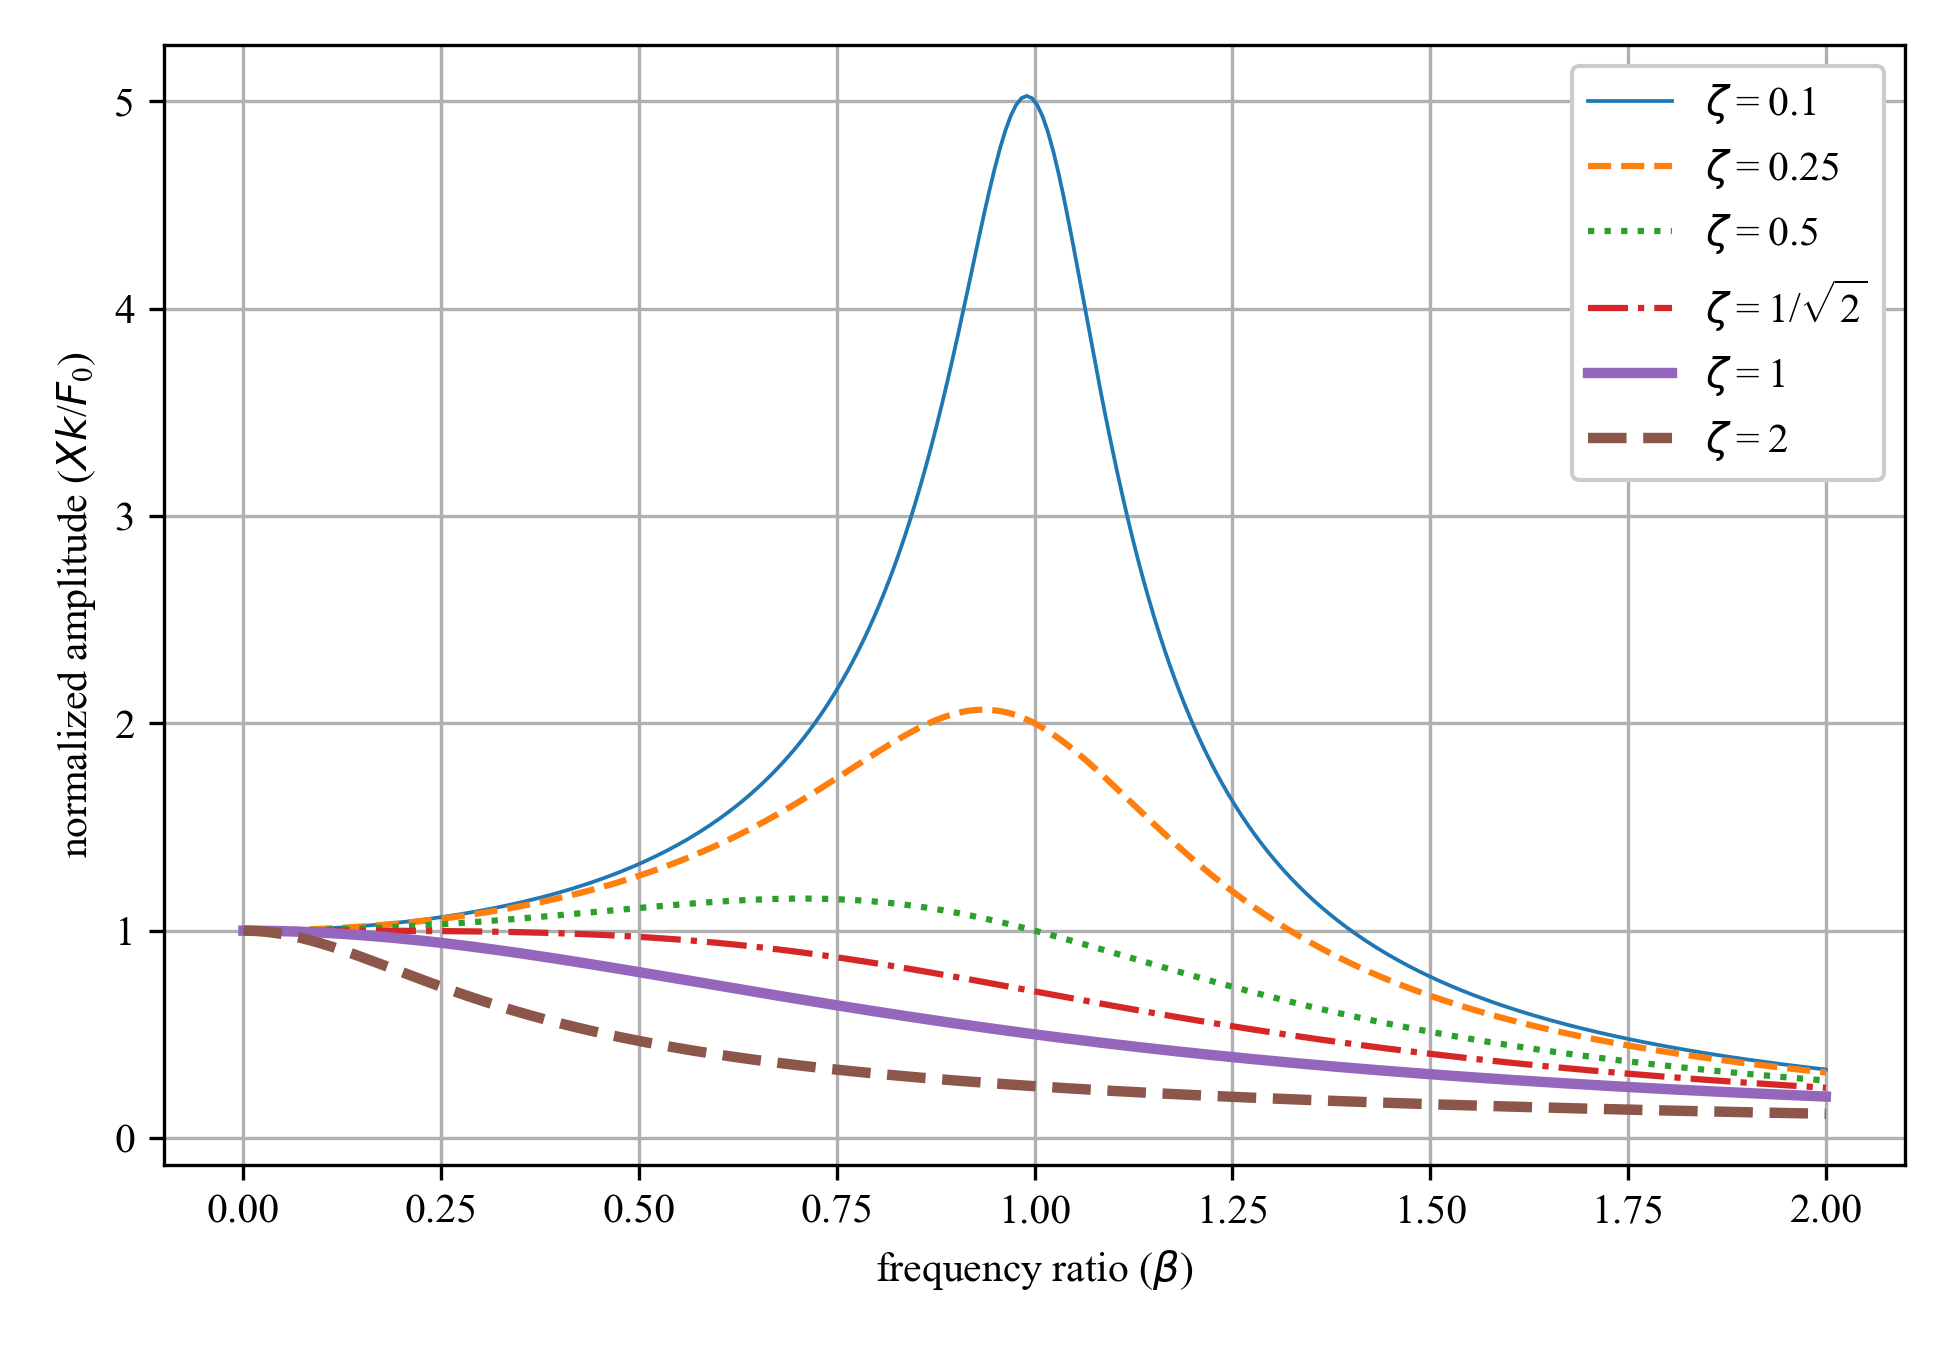
\includegraphics[]{../figures/underdamped_frequency_response_amplitude.png}
				\caption{Normalized amplitude response for frequency ratio ($\beta$) from 0 to 2 for a variety of critical damping ratios.}
			\end{figure}			
			\noindent And again, if we plot the values of the phase vs $\beta$ ($\omega/\omega_n$) we obtain:
			\begin{figure}[H]
				\centering
				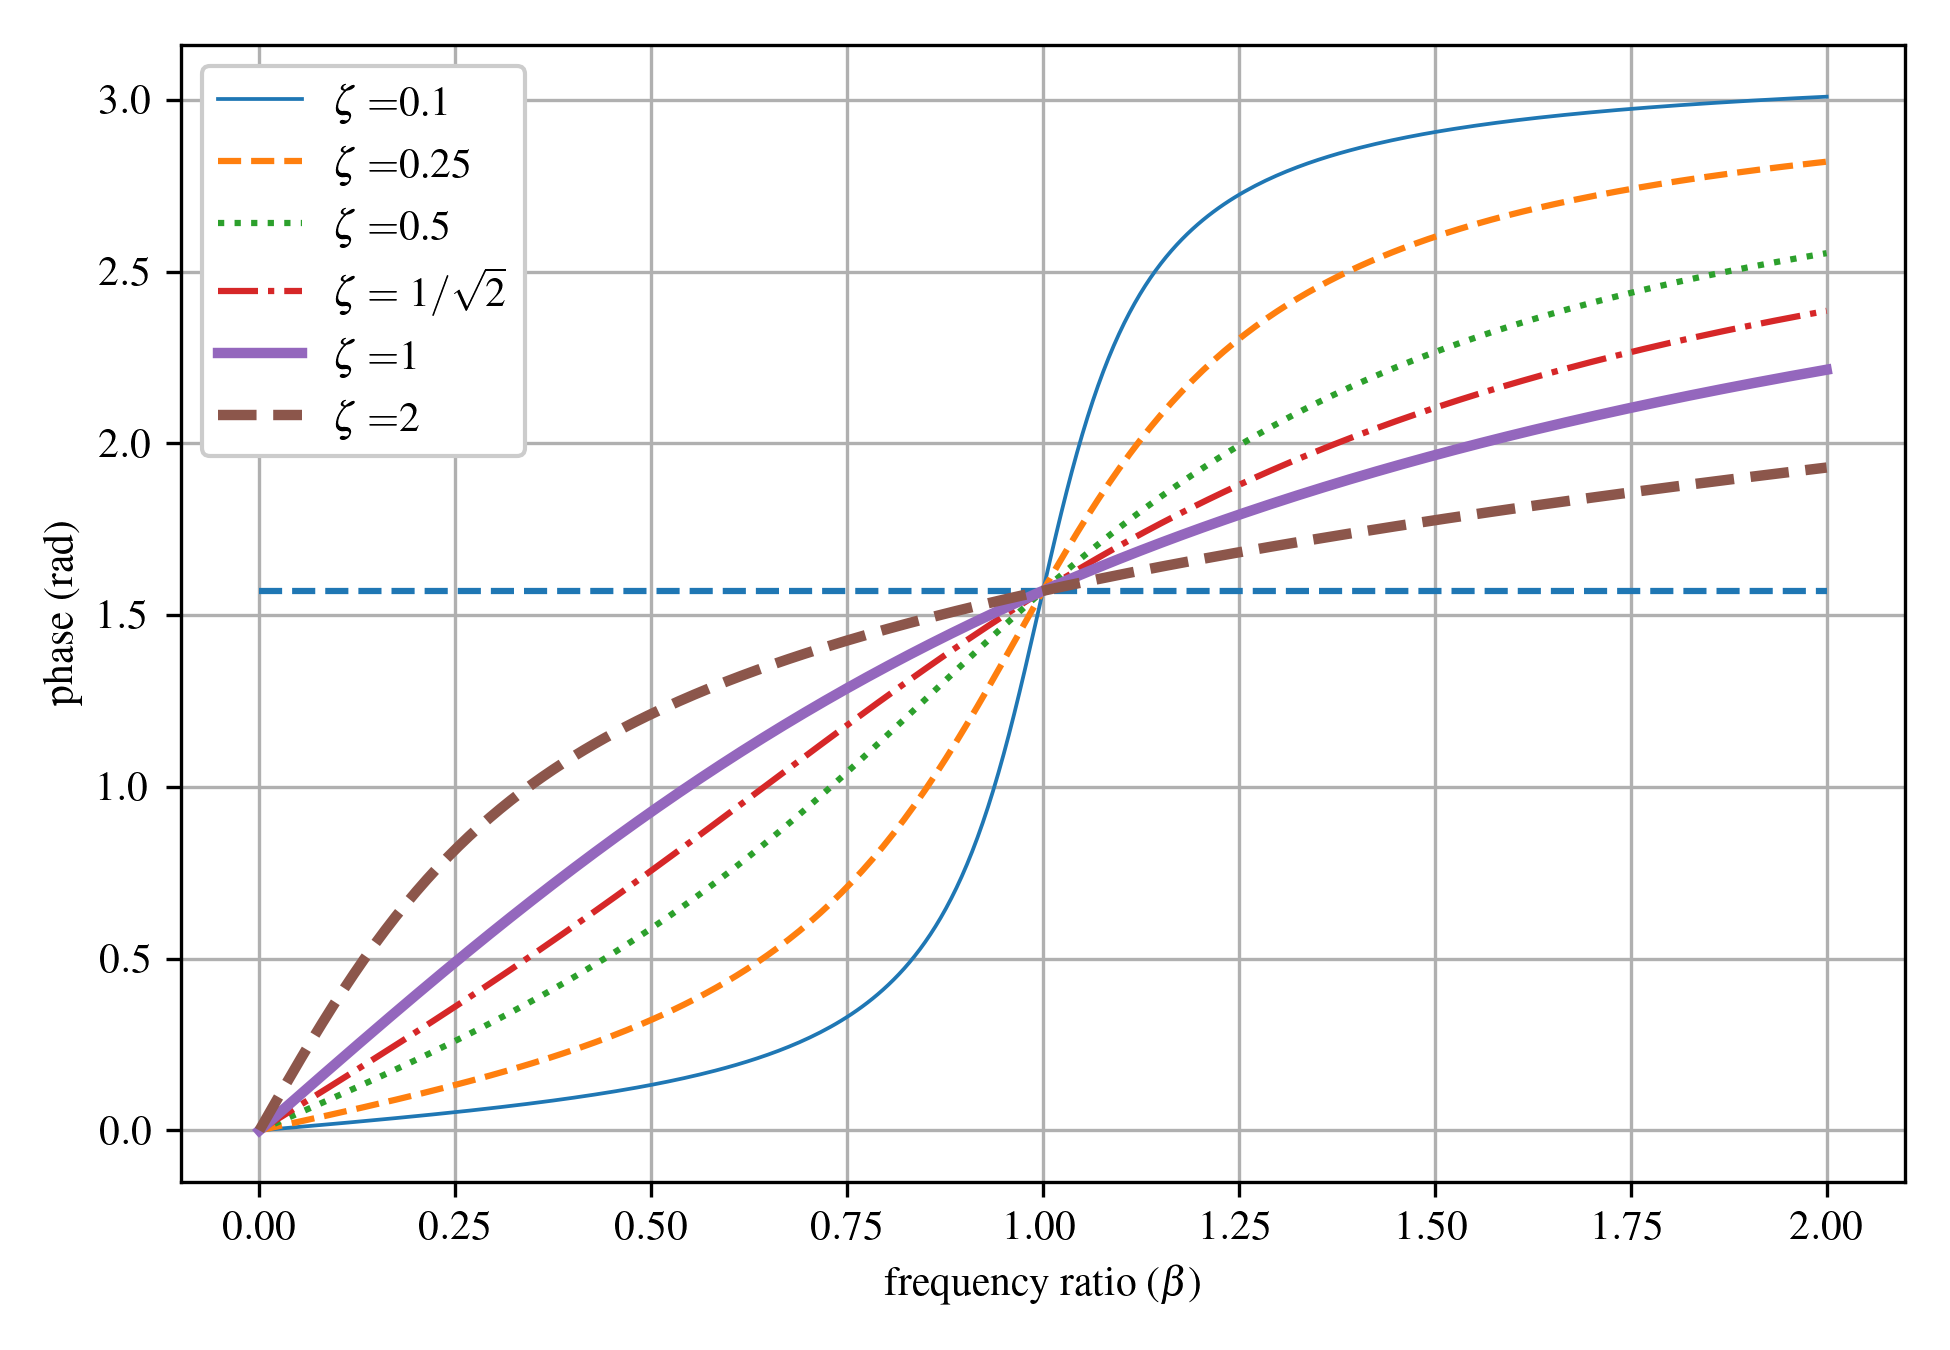
\includegraphics[]{../figures/underdamped_frequency_response_phase.png}
				\caption{Phase response for frequency ratio ($\beta$) from 0 to 2 for a variety of critical damping ratios.}
			\end{figure}				
			\noindent note that the dashed black line is there because the phase values after $\pi/2$ need to be adjusted to obtain a continuous plot. An astute observer would notice that the maximum amplitude is not at $\omega = \omega_n$. While resonance is defined as $\omega = \omega_n$, this does not define the point of maximum displacement of the steady state response. Let us solve for the frequency ratio with the maximum displacement. This will happen when
			\begin{equation}
				\frac{d}{dr}\Bigg(\frac{Xk}{F_0} \Bigg)= 0
			\end{equation}				
			We can show that:
			\begin{equation}
			\Bigg(\frac{1}{\sqrt{(1-\beta^2)^2+(2\zeta \beta)^2}}\Bigg)	\frac{d}{dr} =0
			\end{equation}	
			when 
			\begin{equation}
			\beta_{\text{peak}} = \sqrt{1-2 \zeta^2}= \frac{\omega_p}{\omega_n}, \hspace{1cm} \zeta<1/\sqrt{2} 
			\end{equation}				
			however, this is only true for under damped system in which $\zeta<1/\sqrt{2}$. If $\zeta>1/\sqrt{2}$ than the value in imaginary and the peak value is at $r=0$. In these cases, the maximum displacement is a function of only $\omega_n$. $\omega_p$ represents the driving frequency that correspond to the maximum amplitude ($\frac{Xk}{F_0}$) and is called the \textbf{peak frequency}, and can be calculated as:
			\begin{equation}
			\omega_p = \omega_n \beta_{\text{peak}} = \omega_n \sqrt{1-2 \zeta^2}, \hspace{1cm} \zeta<1/\sqrt{2} 
			\end{equation}				
			
			
			
\begin{example}

			Consider the simple spring mass system, 
			\begin{figure}[H]
				\centering
				\includegraphics[]{../figures/1-DOF-spring_dashpot_mass_horizontal_forced.png}
				\caption{Damped 1-DOF spring-mass system subjected to an external force $F(t)$.}
			\end{figure}				
			\noindent where $\omega_n = 132$ rad/sec and $\zeta$ = 0.0085. Calculate the displacements of the steady-state response for $\omega$=132 and 125 rad/sec. In both cases, use $f_0$ = 10 N/kg. 

			\noindent\textbf{Solution:}	From before, we know the solution for the displacement of the particular solution for $\omega$=132 rad/sec is:
			\begin{equation}
				X = \frac{f_0}{\sqrt{(\omega_n^2 - \omega^2)^2 +  (2\zeta \omega_n \omega)^2}} = \frac{10}{2(0.0085)(132)^2} = 0.034 \text{ m}
			\end{equation}							
			while for $\omega$=125 rad/sec X is:
			\begin{equation}
				X = \frac{f_0}{\sqrt{(\omega_n^2 - \omega^2)^2 +  (2\zeta \omega_n \omega)^2}} = \frac{10}{\sqrt{(1799)^2 +  (280.5)^2}}  = 0.005 \text{ m}
			\end{equation}				
			Therefore, a slight change in the driving frequency (about 5\%) results in a 85\% change in the amplitude of the steady-state response. 
\end{example}

\begin{example}

		

			The steady state response for an engineered system must not surpass 1 cm, if the system can be modeled as the spring and mass system below, what value of $c$ must be used?  
			\begin{figure}[H]
				\centering
				\includegraphics[]{../figures/1-DOF-spring_dashpot_mass_horizontal_forced.png}
				\caption{Damped 1-DOF spring-mass system subjected to an external force $F(t)$.}
			\end{figure}	
			\noindent Use $k$ = 2000 N/m, $m$ = 100 kg, $F(t)$ = 20 cos($6.3t$) N. 			

			\noindent\textbf{Solution:} The steady state solution is:
			\begin{equation}
				x_p(t) = X \text{cos}(\omega t - \phi_p)
			\end{equation}			 
			knowing the amplitude is controlled by $X$: 
			\begin{equation}
				X = \frac{f_0}{\sqrt{(\omega_n^2 - \omega^2)^2 +  (2\zeta \omega_n \omega)^2}} 
			\end{equation}	
			and recalling from the EOM in standard form that $2\zeta \omega_n = c/m$ we can obtain:
			\begin{equation}
				X = \frac{f_0}{\sqrt{(\omega_n^2 - \omega^2)^2 +  (\frac{c}{m} \omega)^2}} 
			\end{equation}		
			rearranging for $c$ gives:		
			\begin{equation}
				c = m\sqrt{\frac{f_0^2}{\omega^2 X^2}-\frac{\big(\omega_n^2-\omega^2\big)^2}{\omega^2}} = \sqrt{\frac{F_0^2}{\omega^2 X^2}-m^2\frac{\big(\omega_n^2-\omega^2\big)^2}{\omega^2}} 
			\end{equation}
			Therefore, if we set $X=0.01$ m we can solve the above equation to yield $c$ = 55.7 kg/s.
			
\end{example}	


	
		\subsection{Base Excitation}

			Often, loading is not applied directly to the mass, but rather the mass of the system is excited when the base of mount that it is attached to is excited. This is called base excitation, or sometimes support motion. Examples of base excitation, or where base excitation is considered, include:
			
			\begin{itemize}
			\item machines on rubber mounts
			\item automobiles excited by the road
			\item building under earthquake loading
			\item hospital equipment
			\end{itemize}
			
			Consider the following system base excited system
			\begin{figure}[H]
				\centering
				\includegraphics[]{../figures/1_DOF_spring_dashpot_mass_vertical_base_excited_FBD.png}
				\caption{Damped 1-DOF spring-mass system subjected to a displacement controlled base excitation showing the FBDs for the equilibrium and displaced positions.}
				\label{fig:1_DOF_spring_dashpot_mass_vertical_base_excited_FBD}
			\end{figure}
			where $x$ is the displacement of the mass and $y$ is the displacement of the base. Note that we consider positive upward here. The EOM can be constructed the same as before, but now considering that the displacement of the springs and damper is $x-y$.  In the equilibrium state, where a positive $x$ is up and the base displaces down:
			\begin{equation}
			\sum F_x = -k\delta -mg =0
			\end{equation}	
			Note that these are both negative because the base displacing down ``pulls'' the mass down with a force $k\delta$ (i.e. if you hold the mass and let the base ``fall''). Conversely, the equation for the displaced state is:
			\begin{equation}
			\sum F_x = -k(\delta + x - y) -mg -c(\dot{x} -\dot{y})
			\end{equation}	
			Apply Newton's second law about the mass ($m\ddot{x}$) of motion to the sum of forces for the displaced position we get:
			\begin{equation}
			\sum F_x = m\ddot{x} = -k\delta -kx + ky -mg -c\dot{x} +c\dot{y}
			\end{equation}	
			applying the equation $-k\delta -mg =0$, and rearrange into the EOM yields:	
			\begin{equation}
			m\ddot{x} + c\dot{x} + kx = c\dot{y} + ky 
			\end{equation}
			Now as before we assume an input for the base excitation. For simplicity we assume:
			\begin{equation}
			y(t) = Y\text{sin}(\omega_b t)
			\end{equation}
			Taking the derivative of the assumed input yields:
			\begin{equation}
			\dot{y}(t) = Y \omega_b \text{cos}(\omega_b t)
			\end{equation}
			where $Y$ is the amplitude and $\omega_b$ is the frequency of the base excitation. Adding these terms into our EOM yields:
			\begin{equation}
			m\ddot{x} + c\dot{x} + kx = c Y \omega_b \text{cos}(\omega_b t)  + k Y\text{sin}(\omega_b t)  
			\end{equation}
			We can get this in standard form if we divide by $m$ and apply the equations for the critical damping ratio and natural frequency:
			\begin{equation}
			\ddot{x} + 2 \zeta \omega_n \dot{x} + \omega_n^2x = 2 \zeta \omega_n \omega_b Y \text{cos}(\omega_b t)  + \omega_n^2 Y\text{sin}(\omega_b t)
			\label{eq:standard_form_base_excitation}  
			\end{equation}
			This equation can be related to a spring-mass-damper system with two harmonic inputs, one cos and one sin as shown below:
			\begin{equation}
			\ddot{x} + 2 \zeta \omega_n \dot{x} + \omega_n^2x = C \text{cos}(\omega_b t)  + D \text{sin}(\omega_b t)  
			\label{eq:standard_form_base_excitation_CD}
			\end{equation}
			where C and D are arbitrary coefficients. 

	
			\subsubsection{Displacement Transmissibility Solution for Base Excitation}
				The steady-state solution is often of more important than the transient solution when designing systems for continuous use. The particular solution for the base excited system annotated in figure \ref{fig:1_DOF_spring_dashpot_mass_vertical_base_excited_FBD} with the EOM presented in equation \ref{eq:standard_form_base_excitation_CD} can be expressed as $	x_p(t)$. To solve for this expression we will use the linearity of the system and solve for a solution that is the sum of two particular solutions. Resulting in:
				\begin{equation}
				 x_p(t) = 	x_p^{(1)}(t) + 	x_p^{(2)}(t)  
				\end{equation}
				
				 Recall that the steady state solution for a harmonically excited spring-mass-damper can be expressed as $x_p(t) = X\text{cos}(\omega t - \phi_p)$, as denoted in equation~\ref{eq:x_p(t)}. For the base excitation problem, we will convert this expression to $x_p(t) = X\text{cos}(\omega_b t - \phi_1)$. Therefore, for a base excited problem, the forcing function can be expressed as the sum of particular solutions:
				\begin{equation}
					C \text{cos}(\omega_b t)  + D \text{sin}(\omega_b t)   = x_p = 	x_p^{(1)} + 	x_p^{(2)} 
				\end{equation}
				where we dropped the $(t)$ term from the expression for simplicity in writing and:
				\begin{equation}
					x_p^{(1)} = X^{(1)}\text{cos}(\omega_b t - \phi_1)
				\end{equation}
				\begin{equation}
					x_p^{(2)} = X^{(2)} \text{sin}(\omega_b t - \phi_1)
				\end{equation}
				Note that $x_p^{(1)}$ uses a cos term while $x_p^{(1)}$ uses a sin term. Both solutions use $\phi_1$ as the damping term as the phase angle is independent of the excitation amplitude and the sin and cos terms account for the difference in phase. 
				
				For $x_p^{(1)}$, we use the method of undetermined coefficients to obtain a solution for $x_p^{(1)} = X^{(1)}\text{cos}(\omega_b t - \phi_1)$. This can be as simple as setting $2 \zeta \omega_n \omega_b Y$ equal to $f_0$ from equation \ref{eq:X_damped} that defines $X$ for underdamped systems. Again, $2 \zeta \omega_n \omega_b Y$  comes from the EOM in standard form as presented in equation 	
				\ref{eq:standard_form_base_excitation}. We can do this because both terms can be considered a ``driving force''. This results in the equation:
				\begin{equation}
					x_p^{(1)} = \frac{2 \zeta \omega_n \omega_b Y}{\sqrt{(\omega_n^2 - \omega_b^2)^2 +  (2\zeta \omega_n \omega_b)^2}}  \text{cos}(\omega_b t - \phi_1)
					\label{eq:xp_1}
				\end{equation}
				where:
				\begin{equation}
					\phi_1 = \tan^{-1} \bigg(\frac{2\zeta \omega_n \omega_b}{\omega_n^2 - \omega_b^2}\bigg)
				\end{equation}
				
				Next, the particular solution associated with $x_p^{(2)} = X^{(2)} \text{sin}(\omega_b t - \phi_1)$ can be obtained using the same method of undetermined coefficients an setting $f_0$ from equation \ref{eq:X_damped} to the driving force for $x_p^{(2)}$ in equation  \ref{eq:standard_form_base_excitation}, $\omega_n^2$. This results in:
				\begin{equation}
					x_p^{(2)} = \frac{\omega_n^2 Y}{\sqrt{(\omega_n^2 - \omega_b^2)^2 +  (2\zeta \omega_n \omega_b)^2}}  \text{sin}(\omega_b t - \phi_1)
					\label{eq:xp_2}
				\end{equation}
				As both equation \ref{eq:xp_1} and \ref{eq:xp_2}  have the same argument $(\omega_b t - \phi_1)$, these can be added as:
				\begin{equation}
					x_p = 	x_p^{(1)} + x_p^{(2)}
				\end{equation}
				to obtain:
				\begin{equation}
					x_p = 	\omega_n Y   \sqrt{\frac{\omega_n^2 + (2 \zeta \omega_b)^2 }{(\omega_n^2 - \omega_b^2)^2 +  (2\zeta \omega_n \omega_b)^2} }  \text{cos}(\omega_bt - \phi_1 - \phi_2)
				\end{equation}
				and:
				\begin{equation}
					\phi_2 = \tan^{-1} \bigg(\frac{\omega_n}{2\zeta \omega_b}\bigg)
				\end{equation}
				where $\phi_2$ is added to account for the cos and sin terms being combined. Again, the $(t)$ has been dropped for simplicity. 
				
				As before, if we want to investigate how a frequency input will affect the response (frequency response) we can substitute substitute 
				\begin{equation}
				\beta=\frac{\omega_b}{\omega_n}
				\end{equation} 
				into the temporal response to obtain:
				\begin{equation}
				X = Y \sqrt{\frac{1+(2 \zeta \beta)^2}{(1-\beta^2)^2 + (2 \zeta \beta )^2}} 
				\end{equation} 
				Next, if we divide by $Y$ we can obtain a normalized expression for the displacement:
				\begin{equation}
				\frac{X}{Y} = \sqrt{\frac{1+(2 \zeta \beta)^2}{(1-\beta^2)^2 + (2 \zeta \beta )^2}} 
				\end{equation} 
				Plotting this for several critical damping ratios:
				\begin{figure}[H]
					\centering
					\includegraphics[]{../figures/base_excitation_displacement_transmissibility.png}
					\caption{Displacement transmissibility for an underdamped 1-DOF system.}
				\end{figure}
				Around resonance, the maximum amount of displacement is transmitted to the mass. Additionally,  the above plot shows that at $\beta=\sqrt{2}$ the displacement transmissibility $X/Y$ is 1. Note the ``flip'' where overdamped systems have a greater response to excitations after $\beta=\sqrt{2}$ than do underdamped systems.

				\begin{example}
	
					A very common example of base motion is the SDOF model of a vehicle wheel driving over a ``rough'' road as shown below. 
					\begin{figure}[H]
						\centering
						\includegraphics[]{../figures/vehicle_on_road_example.png}
					\end{figure}				
					\noindent where $k$ = 400,000 N, $m$ = 1007 kg, $c$ = 20,000 kg/s, the period of road roughness = 6 m, and the height of road roughness = 0.02 m. What is the deflection experience by the car at $v$ = 20 km/h?
					
					\noindent\textbf{Solution:} The road is applying a base excitation that can be approximated as 
					\begin{equation}
						Y = 0.01 \text{ m}
					\end{equation} 				
					\begin{equation}
						v \text{ m/s} = 20 \text{ km/hr}\Bigg(\frac{1000 \text{ m}}{1 \text {km}}\Bigg) \Bigg(\frac{1 \text{ hours}}{3600 \text { s}}\Bigg) = \frac{50}{9} \text{ m/s} = 5.555 \text{ m/sec}
					\end{equation} 	
					\begin{equation}
						\omega_b = \Bigg(\frac{ 5.55 \text{ m}}{s}\Bigg) \Bigg(\frac{ 1 \text{ cycle}}{6 \text{ m}}\Bigg) \Bigg(\frac{ 2 \pi \text{ rad}}{\text {cycle}}\Bigg) = \frac{ 11.11 \pi }{6 } \text{ rad/s} =5.817 \text{ rad/s} 
					\end{equation} 	
					Therefore, the sinusoidal for the base excitation is then:
					\begin{equation}
						y(t) = (0.01) \text{sin}(5.817 t)
					\end{equation} 	
					Next, we can calculate the natural frequency:
					\begin{equation}
						\omega_n = \sqrt{\frac{k}{m}} = \sqrt{\frac{400,000}{1007}} = 19.93 \text{ rad/s}
					\end{equation} 			
					Therefore:
					\begin{equation}
					r=\frac{\omega_b}{\omega_n} = \frac{5.817}{19.93} =0.292
					\end{equation} 		
					and:
					\begin{equation}
					\zeta = \frac{c}{2\sqrt{km}}= \frac{20,000}{2\sqrt{1007\cdot400,000}} = 0.498
					\end{equation}	
					Then it can be found that the maximum deflection of the car is:
					into the temporal response to obtain:
					\begin{equation}
					\begin{split}
					X = Y \sqrt{\frac{1+(2 \zeta r)^2}{(1-r^2)^2 + (2 \zeta r )^2}} = Y \sqrt{\frac{1+(2 \cdot 0.498 \cdot 0.292)^2}{(1-0.292^2)^2 + (2 \cdot 0.498 \cdot 0.292 )^2}}  \\ = 0.0108 \text{ m}
					\end{split}
					\end{equation} 		
				\end{example}	
					
			\subsubsection{Force Transmissibility Solution for Base Excitation}
			
				For some systems, such as those with weak connections, the force transmitted to the mass is more important than the displacement of the mass. The force transmitted to the mass are the sums of the forces applied by the spring and damper. From the FBD above,
				\begin{equation}
				F(t) = k(x-y) + c(\dot{x} - \dot{y}) 
				\end{equation}
				where this force is counteracted by the inertial force of the mass:
				\begin{equation}
				F(t) = -m\ddot{x}(t)
				\end{equation}
				Only considering the steady state we found that 
				\begin{equation}
					x_p(t) = 	\omega_n Y   \sqrt{\frac{\omega_n^2 + (2 \zeta \omega_b)^2 }{(\omega_n^2 - \omega_b^2)^2 +  (2\zeta \omega_n \omega_b)^2} }  \text{cos}(\omega_bt - \phi_1 - \phi_2)
				\end{equation} 
				if we differentiate this twice, to obtain $\ddot{x}(t)$ and combine this with $F(t) = -m\ddot{x}(t)$ we get:
				\begin{equation}
					F(t) = 	m \omega_b^2 \omega_n Y   \sqrt{\frac{\omega_n^2 + (2 \zeta \omega_b)^2 }{(\omega_n^2 - \omega_b^2)^2 +  (2\zeta \omega_n \omega_b)^2} }  \text{cos}(\omega_bt - \phi_1 - \phi_2)
				\end{equation} 
				where the negative sign $F(t) = -m\ddot{x}(t)$ as the force transmitted to the mass is both positive and negative and we are solving for the amplitude of the transmitted force. Again applying:
				\begin{equation}
					\beta=\frac{\omega_b}{\omega_n}
				\end{equation} 
				this becomes:
				\begin{equation}
					F(t) = 	F_\text{T} \text{cos}(\omega_bt - \phi_1 - \phi_2)
				\end{equation} 
				where $F_T$ is the magnitude of the transmitted force and is 
				\begin{equation}
					F_\text{T} = kYr^2 \sqrt{\frac{1+(2 \zeta \beta)^2}{(1-\beta^2)^2 + (2 \zeta \beta )^2}} 
				\end{equation}
				Again, this can be converted to a force transmissibility to provide a normalized response such that:
				\begin{equation}
					\frac{F_\text{T}}{kY} = \beta^2 \sqrt{\frac{1+(2 \zeta \beta)^2}{(1-r^2)^2 + (2 \zeta \beta )^2}} 
				\end{equation}
				Plotting this for several critical damping ratios:
				\begin{figure}[H]
					\centering
					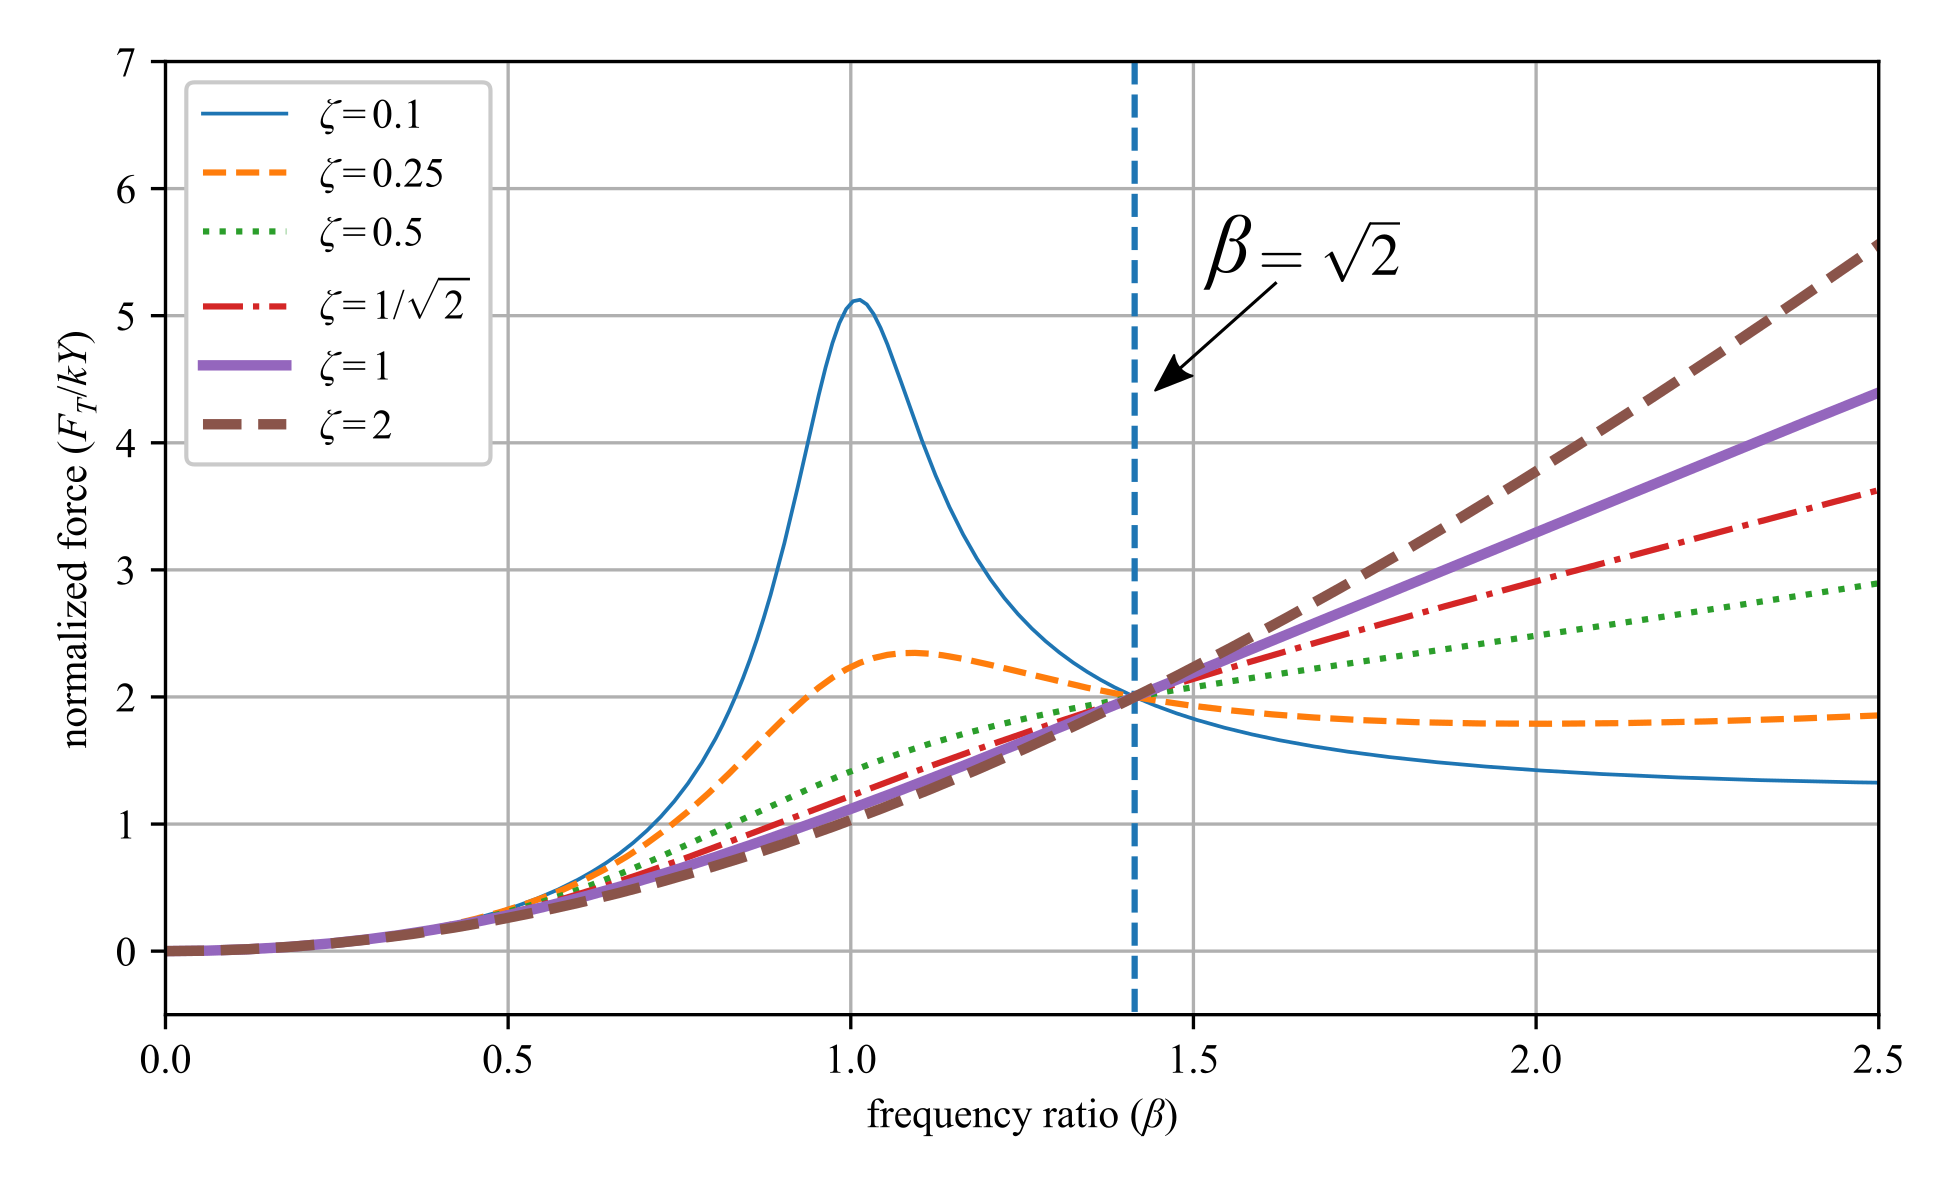
\includegraphics[]{../figures/base_excitation_force_transmissibility.png}
					\caption{Force transmissibility for an underdamped 1-DOF system.}
				\end{figure}
				Again, note the key location $\beta=\sqrt{2}$. At $\beta=\sqrt{2}$ the force transmitted to the system is 2 $\frac{F_\text{T}}{kY}$. However, also note that the normalized force does not necessarily fall off for $\beta$ values greater than $\beta=\sqrt{2}$.  
	
				\begin{example}
					
					For the system given below and excited at the base, should the system be excited above or below the natural frequency if the transmitted force is the design limitation? Consider the under damped with $\zeta=0.1$, and the over damped with $\zeta=2$ conditions. 
		
					\begin{figure}[H]
						\centering
						\includegraphics[]{../figures/1_DOF_spring_dashpot_mass_vertical_base_excited.png}
						\caption{Force transmissibility for an underdamped 1-DOF system.}
					\end{figure}		
				
					\noindent\textbf{Solution:} We can plot the transmissibility of both the force and displacement onto one plot. For $\zeta=0.1$
					\begin{figure}[H]
						\centering
						\includegraphics[]{../figures/base_excitation_force_and_displacement_transmissibility_1.png}
						\caption{Force and displacement transmissibility for the considered base excited system with $\zeta=0.1$.}
					\end{figure}
					it is clear that to minimize the force, the system should be driven with a frequency below the natural frequency. Next for  $\zeta=2$:
					\begin{figure}[H]
						\centering
						\includegraphics[]{../figures/base_excitation_force_and_displacement_transmissibility_2.png}
						\caption{Force and displacement transmissibility for the considered base excited system with $\zeta=2$.}
					\end{figure}			
					it can be seen that the same rationale applies. Therefore, for both $\zeta=0.1$ and $\zeta=2$ the system should be excited below the natural frequency.
				
				\end{example}
	
			
							
				\begin{example}
		
					A single story building is subjected to a harmonic ground motion, $\ddot{y}(t) = A \text{cos}(\omega_b t)$. a) Find the steady-state solution for the structure.  b) If a damper was added between the base and the floor, and $r=2$, what would be the ideal critical damping coefficient to insure the safety of the building. (Think of safety as limiting displacement and transmitted force.) 
					\begin{figure}[H]
						\centering
						\includegraphics[width=0.35\textwidth]{../figures/base_excited_structure.png}
					\end{figure}				
								
					\noindent\textbf{Solution (a):}
						
					For simplicity, we can rearrange the system as what follows:
					\begin{figure}[H]
						\centering
						\includegraphics[width=0.35\textwidth]{../figures/base_excited_structure_simple.png}
					\end{figure}			
		
					solving for the EOM yields:
					\begin{equation}
						m\ddot{x} + kx = ky
					\end{equation} 				
					Notice that this is the same as the EOM for a damped 1-DOF system if $c=0$.	
					\begin{equation}
					m\ddot{x} + c\dot{x} + kx = + c\dot{y} + ky \rightarrow m\ddot{x} + kx = ky
					\end{equation}
					Therefore, we can use the solution:
					\begin{equation}
						x_p(t) = 	\omega_n Y   \sqrt{\frac{\omega_n^2 + (2 \zeta \omega_b)^2 }{(\omega_n^2 - \omega_b^2)^2 +  (2\zeta \omega_n \omega_b)^2} }  \text{cos}(\omega_bt - \phi_1 - \phi_2)
					\end{equation}
					where:
					\begin{equation}
						\phi_1 = \tan^{-1} \bigg(\frac{2\zeta \omega_n \omega_b}{\omega_n^2 - \omega_b^2}\bigg)
					\end{equation}	
					\begin{equation}
						\phi_2 = \tan^{-1} \bigg(\frac{\omega_n}{2\zeta \omega_b}\bigg)
					\end{equation}
					Now we have, or can easily get, values for $\omega_n$, $\omega_b$, and $\zeta$. However, we do not have an expression for $Y$. We can extract the displacement (and therefore the $Y$) from the acceleration as:
					\begin{equation}
						\ddot{y}(t) = A \text{cos}(\omega t)
					\end{equation} 				
					\begin{equation}
						\dot{y}(t) = \frac{A}{\omega} \text{sin}(\omega t) + C_1
					\end{equation} 					
					\begin{equation}
						y(t) = - \frac{A}{\omega^2} \text{cos}(\omega t) + C_1t + C_2
					\end{equation} 					
					Resulting in 
					\begin{equation}
						Y = -\frac{A}{\omega^2}
					\end{equation} 			
					
					\noindent\textbf{Solution (b):} From the plots we solved for before, we can see that we want a critical damping coefficient that is as low as possible. This means any damping added to the system will decrease its safety. This may seem counter-intuitive, but this is because we are attempting to drive the structure at a frequency higher than its natural frequency, something that does not commonalty happen. Typically excitations for a structure are well below its natural frequency.  			
				
				\end{example}			
		
\end{document}


























